\documentclass[fleqn]{jbook}
\usepackage{physpub}

\begin{document}

\begin{question}{教育 物理}{}
\begin{subquestions}

\SubQuestion
転がり迫る石の球に追われている人がトロッコに乗って逃げるときに、逃げき
れるか否かを以下の手順で考察しよう。

\begin{subsubquestions}
\SubSubQuestion

勾配$\theta$の斜面を滑らずに転がり落ちる半径$r$、質量$m$、中心のまわり
の慣性モーメント$I$の回転体(円板、球など)の運動を考えよう。重力加速
度を$g$、斜面の回転体におよぼす転がりまさつ力を$F$、回転体の回転角を
$\alpha$、斜面に沿って測った回転体の中心位置を$x$とする。

回転体の運動は以下の連立方程式によって決定される。回転に関する運動方程
式\eqhref{1-2}を与えて方程式を完成させよ。
\begin{eqnarray}
  m\ddot{x}=mg\sin\theta-F \eqname{1-1}
\end{eqnarray}
\begin{eqnarray}
  \eqname{1-2}
\end{eqnarray}
\begin{eqnarray}
\dot{x}=r\dot{\alpha}      \eqname{1-3}
\end{eqnarray}

但し、$\ddot{}\equiv d^2/dt^2,\dot{}\equiv d/dt$である。

\SubSubQuestion
上の方程式\eqhref{1-1},\eqhref{1-2},\eqhref{1-3}を用いて回転体のエネルギー、
\[
  E=\frac{1}{2}m\dot{x}^2+\frac{1}{2}I\dot{\alpha}^2-mgx\sin\theta
\]
が保存することを確認せよ。

\SubSubQuestion
以下の(a)、(b)、(c)に述べる三物体の運動は、$m,I$を適当に定義すると、
問{\bf (i)}の方程式\eqhref{1-1}、\eqhref{1-2}、\eqhref{1-3}に従う。

(a) 一個の車輪を考える。半径は、20cm、質量は40kgであり、車輪の質量分布は一番外側の輪の部分に集中している円環(リング)であるとする。これが斜面をすべらずに転がり落ちる運動を考える。

(b) トロッコを考える。トロッコを、一つの車輪からなり車軸の上に車台が乗っ
ているものとモデル化する。車輪を(a)で考えた円環とし、それが質量の無視
できる円盤により車軸とつながっており、車軸にはトロッコの車台の質量とそ
れに乗った人の質量をあわせた360kgの重量がかかっているとする。車輪は斜
面をすべらずに転がり落ちるとし、車軸のまさつは無視する。

(c)石球を考える。質量$M=2.0\times 10^4$kg、半径$R=$1.0mの石球が斜面を
すべらずに転がり落ちるとする。球の中心のまわりの慣性モーメントは
$\ds{\frac{2}{5}MR^2}$で与えられる。

上の(a)、(b)、(c)のそれぞれの物体の、斜面に沿った方向の加速度を
$g_a,g_b,g_c$とする。勾配30度の斜面を直線状下方に転がる場合に、
$g_a:g_b:g_c$の比を求めよ。

\SubSubQuestion
問{\bf (iii)}の(b)に述べたトロッコが動き始めた時、石球の中心はトロッコ後端から
6.0mのところにあり、秒速3.0mで迫っていた。トロッコの車高は石球の半径に
等しいとすると、石球はトロッコに衝突するかしないかを判定し、後者の場合
には約何mまで接近するかを計算せよ。計算には$g=$9.8m/s$^2$を用いよ。

\end{subsubquestions}

\SubQuestion

\begin{subsubquestions}
\SubSubQuestion
図のように断面積$S$、長さ$L$の円柱導体に一様な定常電流$I$が流れている。
その抵抗$R$は抵抗率$\rho$により$R=\rho L/S$と表せる。この導体中の電流密
度$j$(電流に垂直な単位断面積当たりの電流)はいくらか。また、導体中の
電場$E$と電流密度$j$との関係を導け。

\begin{center}
\includegraphics[clip,height=7mm,width=55mm]{1997phys-1.eps}
\end{center}

\SubSubQuestion
\parbox[t]{110mm}{
球形電極(半径$a$)と球殻電極(半径$b$)が同心に配置されており、それらの間は半径$c$のところで2層の球殻に分けられ($a<c<b$)、内側に抵抗率$\rho_1$の導体、外側に抵抗率$\rho_2$の導体が詰められている(右に断面図を示す)。電極間に電圧をかけ、一様な定常電流$I$を流す。中心からの距離$r$として、以下の問に答えよ。なお、実際上、球に細い穴をあけ中心の電極に導線をつなぐが、その穴と導線の影響は無視できるものとする。また、電極、導線の抵抗率も十分小さく無視できるものとする。}\parbox[t]{50mm}{\vspace*{-5mm}
\begin{center}
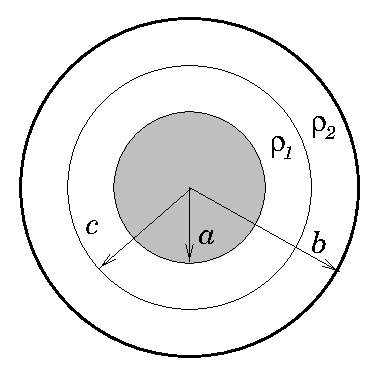
\includegraphics[clip,height=35mm,width=35mm]{1997phys-2.eps}
\end{center}
}

イ) 電流密度$j$、電極間の電場の強さ$E$を$r$の関数で表せ。

ロ)電極間の電圧$V$、抵抗$R$を求めよ。

ハ)中心の電極表面にたまっている全電荷$Q$を求めよ。

ニ)異なる導体の境界面にたまっている全電荷$Q'$を求めよ。

\end{subsubquestions}

\SubQuestion

気体の比熱においては、その体積を一定に保ちながら測る場合の定積比熱
$C_V=(\delta Q/dT)_V$と、圧力を一定に保ちながら測る場合の定圧比熱
$C_p=(\delta Q/dT)_p$とは値が異なる。但し、$T$は温度、$V$は体積、$p$は
圧力、$Q$は熱量である。

\begin{subsubquestions}
\SubSubQuestion
1モルの理想気体の状態方程式を書き、これを用いて理想気体1モルの$C_V$
と$C_p$の関係を導け。但し、気体定数を$R$とせよ。

\SubSubQuestion
理想気体が準静的な断熱変化をするときに
\[ C_V dT+p dV=0 \]
が成り立つことを示せ。

\SubSubQuestion
理想気体が準静的な断熱変化をするときに
\[ pV^{C_p/C_V}= 一定 \]
が成り立つことを示せ。

\SubSubQuestion
ディーゼル機関ではシリンダー内で空気を圧縮して温度を上げ、重油の霧を点
火させる。この圧縮が準静的かつ断熱的に行われ、空気は理想気体であると仮
定しよう。重油の霧の点火温度が627$\degC$の場合、シリンダー内の空気の体積
を何分の一に圧縮させればこの点火温度に達するか、有効数字2桁で計算せよ。
但し圧縮前の空気の温度は27$\degC$であり、空気の比熱比は
$C_p/C_V=\frac{7}{5}$であるとする。

\end{subsubquestions}
\end{subquestions}
\end{question}
\begin{answer}{教育 物理}{}
  \begin{subanswers}
    \SubAnswer

    \begin{subsubanswers}
      \SubSubAnswer
      \[
      I\ddot \alpha = rF
      \]
      
      \SubSubAnswer
      \eqhref{1-1}式に両辺$\dot x$をかけて積分すると、
      \[
      \frac{1}{2}m\dot x^2=mgx\sin\theta-Fx+C_1
      \]
      となる。ただし、$C_1$は積分定数である。同様にして、\eqhref{1-2}式
      に$\dot \alpha$をかけて、\eqhref{1-3}式を使うと、
      \[
      I\ddot\alpha \dot\alpha=rF\dot\alpha=F\dot x \qquad
      \Yueni \frac{1}{2}I\dot \alpha^2=Fx+C_2
      \]
      ただし、$C_2$は積分定数。従って、
      \[
      E=\frac{1}{2}m\dot x^2+\frac{1}{2}I\dot
      \alpha^2-mgx\sin\theta=C_1+C_2=\mbox{一定}
      \]
      
      \SubSubAnswer
      (a)、(b)、(c)それぞれ以下のように$m,I,r$を定義すれば方程式
      \eqhref{1-1}、\eqhref{1-2}、\eqhref{1-3}に従う。
      
      (a) $m=40\Unit{kg},\quad I=1.6\Unit{kgm^2},\quad r=0.2\Unit{m}$
      
      (b) $m=400\Unit{kg},\quad I=1.6\Unit{kgm^2},\quad r=0.2\Unit{m}$
      
      (c) $m=2.0\times 10^4\Unit{kg},\quad I=8.0\times 10^3\Unit{kgm^2},\quad r=1\Unit{m}$
      
      ここで、方程式\eqhref{1-1}、\eqhref{1-2}、\eqhref{1-3}から
      $\alpha,F$を消去すると、
      \[
      m\ddot x+\frac{I}{r^2}\ddot x - mg\sin\theta = 0 \qquad
      \Yueni \ddot x = \frac{1}{1+\frac{I}{mr^2}}g\sin\theta
      \]
      
      $\ddot x$が斜面方向の加速度であるから、(a)、(b)、(c)それぞれの場
      合の値を代入すれば、
      \[
      g_a:g_b:g_c=\frac{1}{2}:\frac{10}{11}:\frac{5}{7}
      \]
      
      \SubSubAnswer
      {\bf(iii)}より、
      \[
      g_b=\frac{10}{11}g\sin\theta=\frac{5}{11}g,\quad
      g_c=\frac{5}{7}g\sin\theta=\frac{5}{14}g
      \]
      $t=0$で石球の中心$x_c=0$、トロッコの後端$x_b=6.0$とすると、
      \[
      x_b=6+\frac{1}{2}g_bt^2,\quad x_c=3.0t+\frac{1}{2}g_ct^2
      \]
      
      従って、石球とトロッコの距離$x_b-x_c-1$を計算すると、
        \[
        x_b-x_c-1=\frac{15}{308}g\left(t-\frac{154}{5g}\right)^2-\frac{462}{10g}+5>0
        \] 
        よって、石球とトロッコは衝突せず、また、もっとも接近す
        るのは、$t=\frac{154}{5g}$のときで、その距離は、約0.3mであ
        る。


    \end{subsubanswers}

    \SubAnswer    
    \begin{subsubanswers}
      \SubSubAnswer
      \[
      j=\frac{I}{S}
      \]
      また、この導体の両端の電圧を$V$とすると、
      \[
      V=EL=IR
      \]
      \[
      \Yueni E=\frac{IR}{L}=\frac{I}{L}\frac{\rho L}{S}=\rho j
      \]

      \SubSubAnswer
      (イ)$j=\frac{I}{4\pi r^2}$
      \[
      E(r) = \rho j = \left\{ \begin{array}{ll}
          \rho_1\frac{I}{4\pi r^2} & a < r < c \\
          \rho_2\frac{I}{4\pi r^2} & c < r < b 
        \end{array} \right.
      \]
      
      (ロ) (イ)の結果より
      \[
      V = \int_a^b E dr =
      \frac{1}{4\pi}\left(\frac{\rho_1}{a} +
      \frac{\rho_2-\rho_1}{c} - \frac{\rho_2}{b}\right) I
      \]
      $V=RI$より
      \[
      R=\frac{1}{4\pi}\left(\frac{\rho_1}{a} +\frac{\rho_2-\rho_1}{c} -
      \frac{\rho_2}{b}\right) 
      \]

      (ハ) ガウスの法則より
      \[
      Q = 4\pi a\varepsilon_0 E(a) = \varepsilon_0\rho_1 I
      \]
      
      (ニ) (ハ)同様、ガウスの法則より
      \[
      Q' = \lim_{r\rightarrow c+0} 4\pi r \varepsilon_0 E(r) - Q =
      \varepsilon_0 I(\rho_2-\rho_1)
      \]

    \end{subsubanswers}

    \SubAnswer
    \begin{subsubanswers}
      
      \SubSubAnswer
      状態方程式は、$pV=RT$ 

      また、$\delta Q = p dV + dU$を用いると、
      \[
      C_V = \left(\frac{\delta Q}{dT}\right)_V = \frac{dU}{dT}
      \]
      \[
      C_p = \left(\frac{\delta Q}{dT}\right)_p =
      \frac{dU}{dT}+p\left(\frac{dV}{dT}\right)_p = \frac{dU}{dT} + R
      \]
      \begin{equation}
      \Yueni C_V+R=C_p \eqname{a3-1}
      \end{equation}

      \SubSubAnswer
      断熱変化なので、$\delta Q=0$。よって
      \begin{equation}
      0 = pdV+dU = pdV+\frac{dU}{dT}dT = pdV + C_VdT \eqname{a3-2}
      \end{equation}

      \SubSubAnswer
      状態方程式および式\eqhref{a3-1}から、
      $Vdp+pdV=RdT=(C_p-C_V)dT$。よって、式\eqhref{a3-2}において
      $dT$を$dp,dV$に置き換えると、
      \[
      C_p pdV + C_V V dp = 0 \qquad \Yueni d\left(pV^{\frac{C_p}{C_V}}\right) 
      = 0
      \]
      \[ 
      \Yueni pV^{\frac{C_p}{C_V}}=\mbox{一定}
      \]

      \SubSubAnswer
      圧縮前の圧力、体積をそれぞれ$p_i,V_i$とし、点火温度に達した
      とき、それぞれ$p_f,V_f$になったとすると、
      \[
      p_i V_i^{\frac{7}{5}} = p_f V_f^{\frac{7}{5}}
      \]
      それぞれの温度での状態方程式から、$p_i,p_f$を消去すると、
      \[
      300 R V_i^{\frac{2}{5}} = 900 R V_f^{\frac{2}{5}}
      \]
      \[
      \Yueni \left(\frac{V_f}{V_i}\right)^{\frac{2}{5}} = \frac{1}{3} \qquad
      \Yueni \frac{V_f}{V_i} = \frac{1}{9\sqrt{3}} \sim
      \frac{1}{16} 
      \]
      したがって、16分の1に圧縮すれば良い。


    \end{subsubanswers}
      

\end{subanswers}
\end{answer}



\end{document}



